\documentclass{standalone}

\usepackage{tikz}
%\usetikzlibrary{arrows}
\usetikzlibrary{shapes.geometric}
\usetikzlibrary{decorations.markings}
\begin{document}
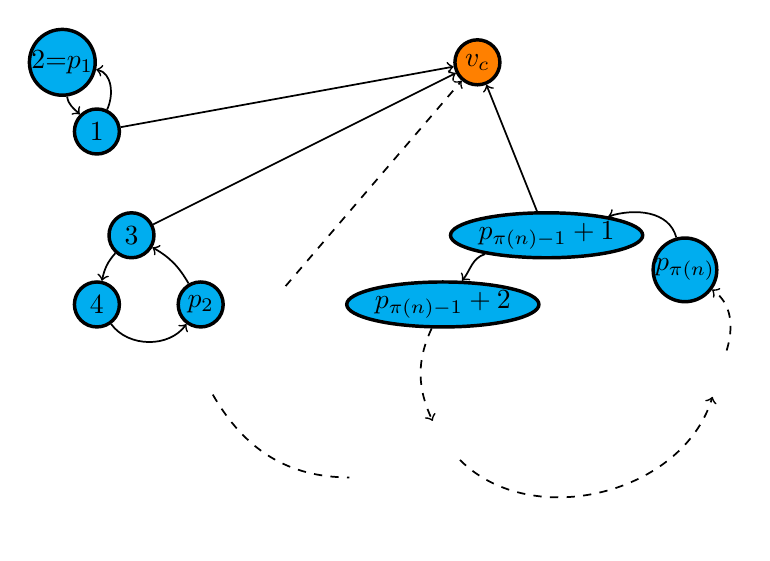
\begin{tikzpicture}
[every node/.style={inner sep=0pt}]
\node (5) [circle, minimum size=16.25pt, fill=cyan, line width=1.25pt, draw=black] at (50.0pt, -87.5pt) {\textcolor{black}{3}};
\node (1) [circle, minimum size=16.25pt, fill=cyan, line width=1.25pt, draw=black] at (37.5pt, -50.0pt) {\textcolor{black}{1}};
\node (6) [circle, minimum size=16.25pt, fill=cyan, line width=1.25pt, draw=black] at (37.5pt, -112.5pt) {\textcolor{black}{4}};
\node (7) [circle, minimum size=16.25pt, fill=cyan, line width=1.25pt, draw=black] at (75.0pt, -112.5pt) {\textcolor{black}{$p_2$}};
\node (8) [circle, minimum size=16.25pt, fill=orange, line width=1.25pt, draw=black] at (175.0pt, -25.0pt) {\textcolor{black}{$v_c$}};
\node (2) [ellipse, minimum size=16.25pt, fill=cyan, line width=1.25pt, draw=black] at (200.0pt, -87.5pt) {\textcolor{black}{$p_{\pi(n)-1}+1$}};
\node (12) [ellipse, minimum size=16.25pt, fill=cyan, line width=1.25pt, draw=black] at (162.5pt, -112.5pt) {\textcolor{black}{$p_{\pi(n)-1}+2$}};
\node (15) [circle, minimum size=16.25pt, fill=white, line width=1.25pt] at (262.5pt, -137.5pt)  {};
\node (13) [circle, minimum size=16.25pt, fill=cyan, line width=1.25pt, draw=black] at (250.0pt, -100.0pt) {\textcolor{black}{$p_{\pi(n)}$}};
\node (14) [circle, minimum size=16.25pt, fill=white, line width=1.25pt] at (162.5pt, -162.5pt)  {};
\node (4) [circle, minimum size=16.25pt, fill=cyan, line width=1.25pt, draw=black] at (25.0pt, -25.0pt) {\textcolor{black}{2=$p_1$}};
\node (16) [circle, minimum size=16.25pt, fill=white, line width=1.25pt] at (75.0pt, -137.5pt)  {};
\node (17) [circle, minimum size=16.25pt, fill=white, line width=1.25pt] at (137.5pt, -175.0pt)  {};
\node (18) [circle, minimum size=16.25pt, fill=white, line width=1.25pt] at (100.0pt, -112.5pt)  {};
%\node (19) [circle, minimum size=16.25pt, fill=white, line width=1.25pt] at (125.0pt, -125.0pt)  {};
\draw [line width=0.625, ->, color=black] (4) to  [in=135, out=278] (1);
\draw [line width=0.625, ->, color=black] (1) to  (8);
\draw [line width=0.625, ->, color=black] (5) to  (8);
\draw [line width=0.625, ->, color=black] (5) to  [in=78, out=228] (6);
\draw [line width=0.625, ->, color=black] (7) to  [in=330, out=120] (5);
\draw [line width=0.625, ->, color=black] (1) to  [in=348, out=65] (4);
\draw [line width=0.625, ->, color=black] (6) to  [in=234, out=306] (7);
\draw [line width=0.625, ->, color=black] (2) to  [in=51, out=197] (12);
\draw [line width=0.625, ->, color=black] (13) to  [in=17, out=105] (2);
\draw [line width=0.625, ->, color=black] (2) to  (8);
\draw [line width=0.625, ->, dashed, color=black] (12) to  [in=115, out=245] (14);
\draw [line width=0.625, ->, dashed, color=black] (15) to  [in=324, out=73] (13);
\draw [line width=0.625, ->, dashed, color=black] (14) to  [in=253, out=315] (15);
\draw [line width=0.625, dashed, color=black] (16) to  [in=180, out=300] (17);
\draw [line width=0.625, ->, dashed, color=black] (18) to  (8);
%\draw [line width=0.625, ->, dashed, color=black] (19) to  (8);

\end{tikzpicture}
\end{document}

